% !TEX encoding = UTF-8
% !TEX TS-program = pdflatex
% !TEX root = ./thesis.tex
% !TEX spellcheck = en

%************************************************

\section{Introduction}
The Web contains a large amount of structured data, most of which represent the main content of web pages. For example, given a Amazon web page that describes a DVD product, provided information about the item, such as prize, title, reviewers, ads, etc. are organized in a structured way. 

Although humans can easily understand how such information are structured (e.g., distinguish between the structured data and the rest of the web content),  machines cannot extract this semantic from
the HTML code.
Nowadays, to solve this issue two main approaches are applied: 
\begin{itemize}
\item Using data markups to encode machine-readable knowledge. These markups are not related to the formatting of data but they just make the metadata and text enclosed within the XHTML tags more meaningful to computers.   
\item Data Mining methods automatically extract structural data based on structural features, visual features or both. 
\end{itemize}
Although using data markups makes web pages machine-readable, there are several reasons why the first solution can not be applied on all websites. First, data intensive websites such as Deep Web Databases (e.g. Amazon.com, Trulia.com) are not favorable to make accessible all their information assets. Another important reason is that enriching web pages with XHTML tags requires human efforts which do not involve direct earnings for organizations' websites.\\
Several methods to extract structured data have been presented in the literature. The first approaches were hand-crafted web scrapers based on regular expressions. An obvious disadvantage of these approaches is that different rule expressions need to be manually created for each website. Furthermore, an individual website may also change its structure or layout over time
making this approach not scalable and in need of continuous maintenance. 
\\
Several supervised and unsupervised Data Mining methods were implemented later ~\cite{Liu2004,miao2009,Lerman2004,Gatterbauer2007,Liu2010}.
Although these methods close the challenge of automatic extraction of structured data from a web page, they fail to detect data record which span multiple web pages. \color{black}This is an open issue, because many websites, especially data-intensive (e.g. Amazon, Trulia, AbeBooks,\ldots), present their listings as \emph{logical list}, that is, a list spanning multiple pages (\textit{e.g.} computers, books, home listings)\footnote{The motivations behind this approach are as well technical (reducing bandwidth and latency), and non technical as avoiding information overload or maximizing page views.}. It is as if, each list represents a \emph{view} of the same \emph{logical list}. Similar to databases, where a \emph{view} can represent a subset of the data contained in a table partitioned over a set of attributes, a \emph{logical list} is split in multiple \emph{views} (web pages) in order to avoid information overload and to facilitate users' navigation. 

\begin{figure}[t!]
\centering
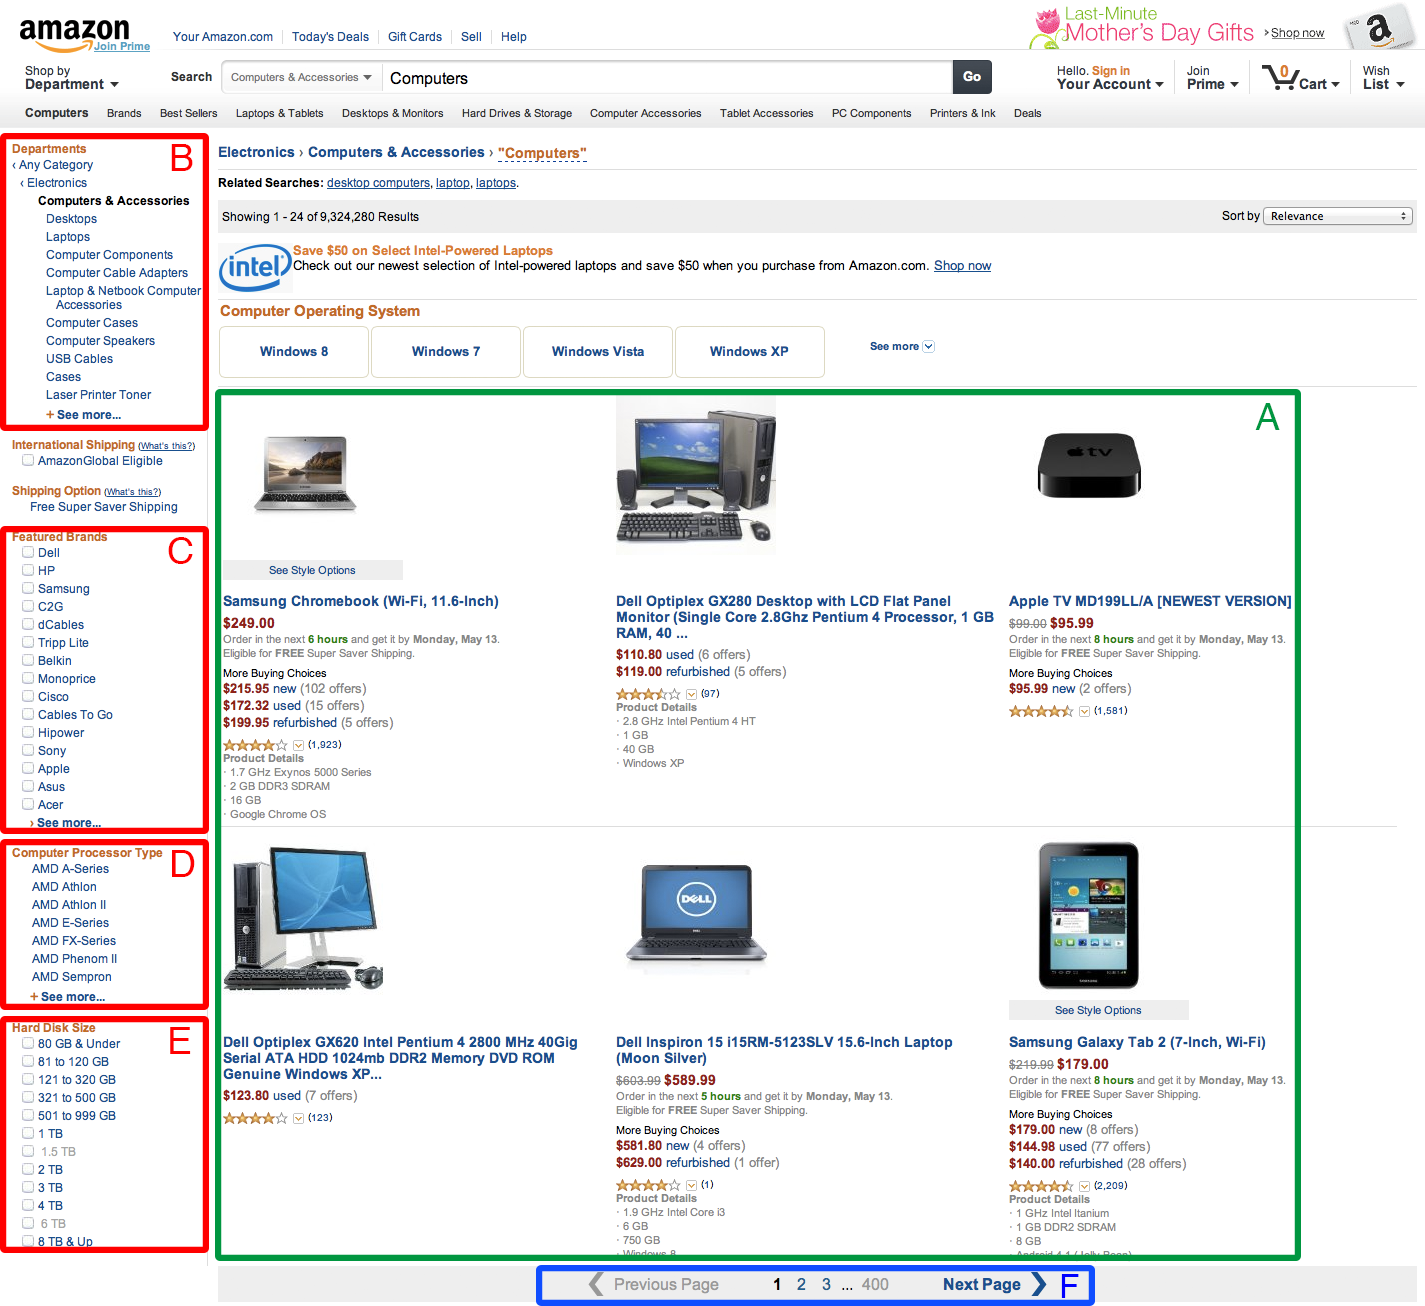
\includegraphics[scale=0.40]{imgs/chap_2/Amazon.png}
\caption{An example of Amazon web page}
\label{fig:amazon}
\end{figure}
For example, Fig.~\ref{fig:amazon} shows a web page from Amazon.com that contains the results for the query ``Computer''.
On this page, the boxes A, B, C, D, E, F are web lists. The list in the box A shows a \emph{view} of the ``Computers'' products, that is the top six sorted by relevance, and F allows us to navigate to the other views of the products ordered by relevance. Thus navigating the links in F we can generate the \emph{logical list} of the products for the query ``Computer''. Boxes B, C, D and E contain respectively the lists representing filters for ``Department'', ``Featured Brands'', ``Computer Processor Type'', and ``Hard Disk Size'', which are attributes of the \emph{virtual} table ``Computer''. Moreover, the anchor-text links in boxes B, C, D and E stores valuable information which can be used to annotate data records, and thus to individuate new attributes. For example, the anchor-text links of web list C can be used to index data records based on ``Computer brands''. Traditionally, search engines use the proximity of terms on a page as a signal of relatedness; in this case the computer brand terms are highly related to some data records, even though they are distant.

Providing automated techniques for \emph{logical list} extraction would be a significant advantage for data extraction and indexing services. Existing data record extraction methods~\cite{Liu2004,miao2009,Gatterbauer2007,Liu2010} focus only in extracting \textit{view} lists, while several commercial solutions\footnote{Lixto, Screen Scraper Studio, Mozenda Screen Scaper} provide hand-coded rules to extract \emph{logical lists}. 

In this chapter, I face this issue by proposing a novel unsupervised algorithm for automatic discovery and extraction of \emph{logical lists} from the Web. This method requires only one page containing a \emph{view list}, and it is able to automatically extract the \emph{logical list} containing the example \emph{view list}. Moreover, during the process, it enriches the list's elements with the pair \emph{$<$url, anchor-text$>$}  used for the extraction task. We have validated our method on a several real websites, obtaining high effectiveness.
\section{Definitions and Problem Formulation}
\label{2Definition}
In this section, I introduce a set of definitions that will be used through the thesis.

A web page is characterized by multiple representations, such as a textual representation (composed by web page terms), a visual representation (composed by information about rendered web page) and a structural representation (composed by HTML tags). For extracting logical lists both the visual and the structural representations are exploited. %For this reason, I provide in the following formal definitions which identify the sources of information exploited by the proposed method.

\begin{definition}
\label{def_chap2:structuralRepresentation}
A web page is characterized by a \textbf{Structural Representation} composed by web elements inscribed in HTML tags and organized in a tree-based structure. HTML tags can be applied to pieces of text, hyperlinks and multimedia data to give them different meaning and rendering in the web page.
\end{definition}
%Although a web page has a structural representation which distinguishes it from a plain and unstructured textual document, a web page can not be considered well structured such as a database because HTML is a language markup projected just for data rendering rather than for storing data such as XML.
 
\begin{definition}
\label{def_chap2:webLayout} The \textbf{ Web Page Rendering} is the process of laying out a spatial position of all the text/images and other web elements in a web page to be rendered.
\end{definition}


 
\begin{definition}
\label{def_chap2:visualRepresentation}
\textbf{Web Page Visual representation.} When a web page is rendered in a web browser (see Def.~\ref{def_chap2:webLayout}), the CSS2 visual formatting model~\cite{WiumLie99} represents the web page's elements by rectangular boxes that are laid out one after the other or nested inside each other by forming a tree, called \textbf{Rendered Box Tree}. By associating the web page with a coordinate system whose origin is at the top-left corner, the spatial position of each web page's element is fully determined by the tuple $(x,y,h,w)$, where $(x, y)$ are the coordinates of the top-left corner of its corresponding box (i.e. the position of the box in the rendered page), and $(h, w)$ are the box's height and width respectively (i.e. the size of the box in the rendered page). Therefore, the \textbf{Visual Representation} of a web page is given by its Rendered Box Tree.
\end{definition}

The rendered box tree can be generated by any web browser which follows W3C specifications for rendering~\cite{WiumLie99}. Moreover, the rendered box tree could have a completely different structure from that of the corresponding HTML tag tree. This because \emph{i) }a web page can be enriched of invisible elements (like the $<$head$>$ tag or elements that have \emph{display:none;} set), and \emph{ii}) the generation of the rendered box tree requires the execution of javascript and css code.
  
 \begin{figure*}
 \center
\subfloat[Box Structure]{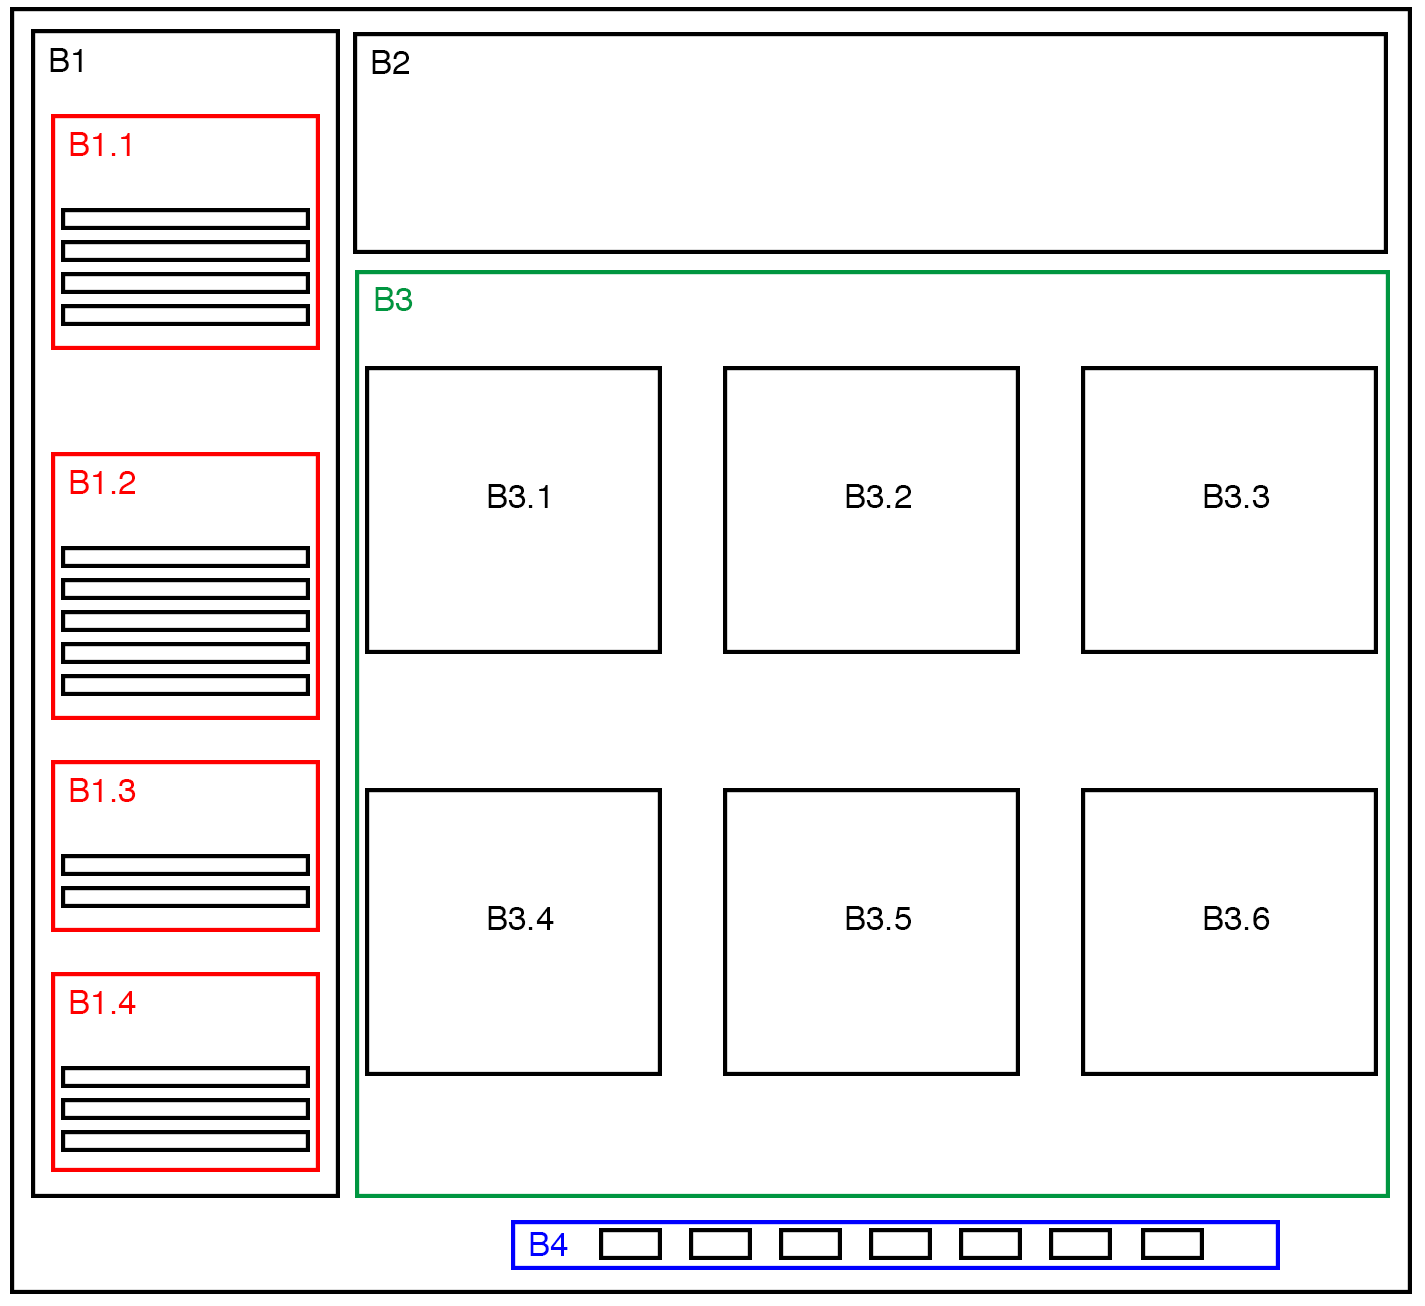
\includegraphics[scale=0.25]{imgs/chap_2/Rendered-box-tree1.png}} 
\subfloat[Rendered Box Tree]{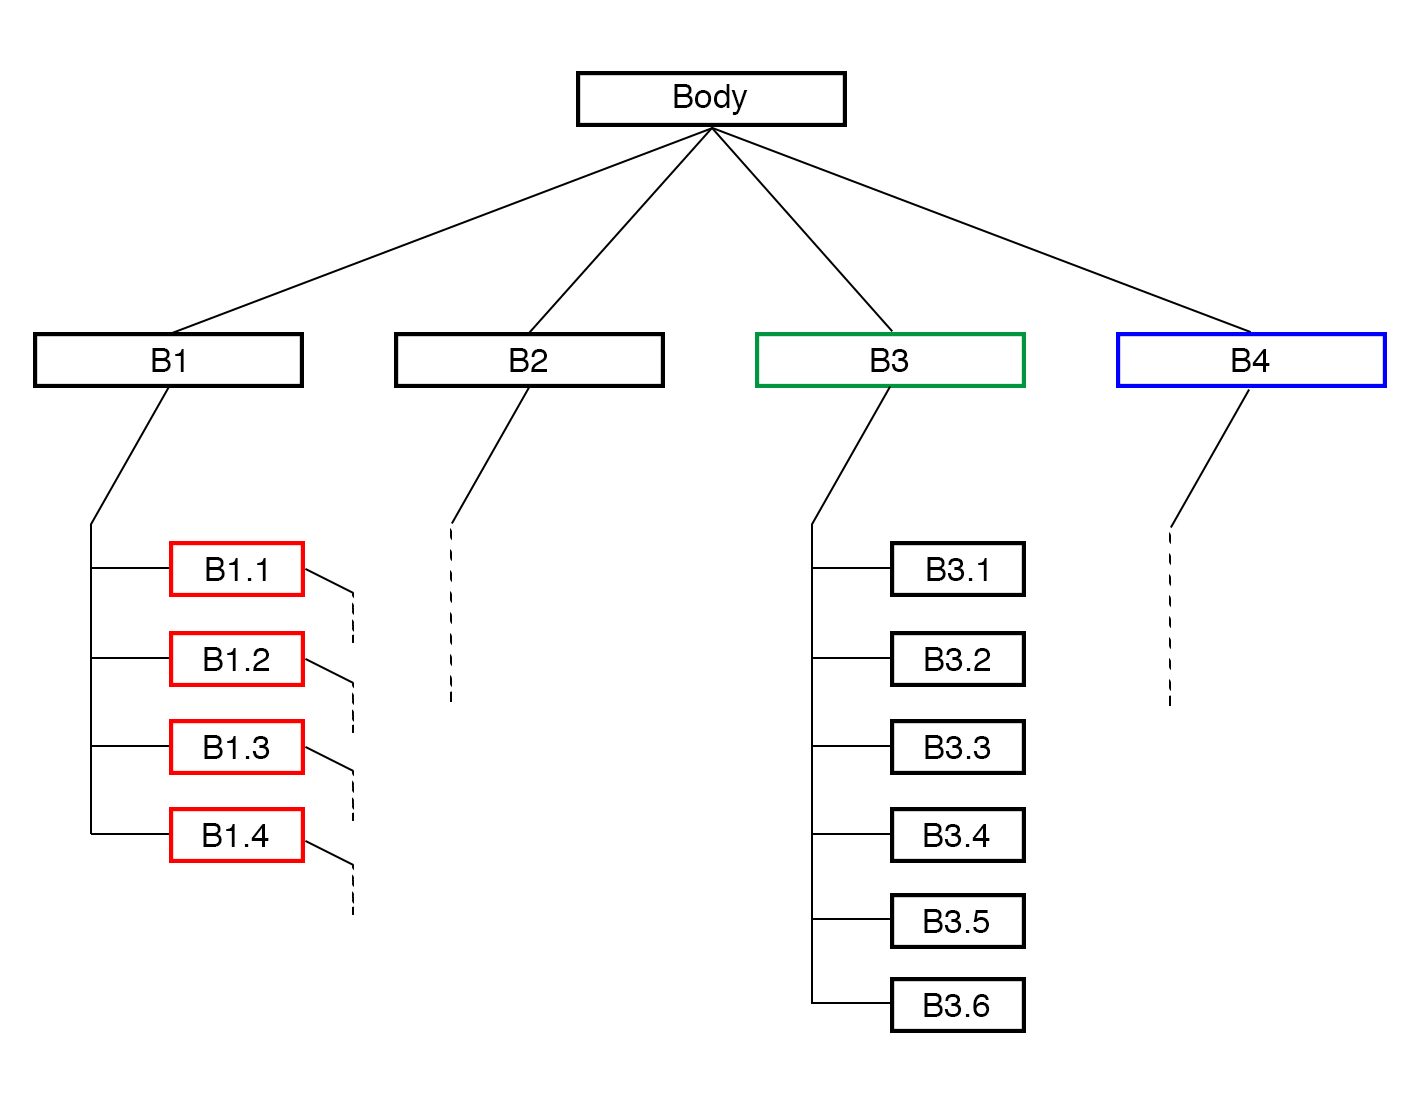
\includegraphics[scale=0.30]{imgs/chap_2/Rendered-box-tree2.png}}\
\subfloat[Structural Representation]{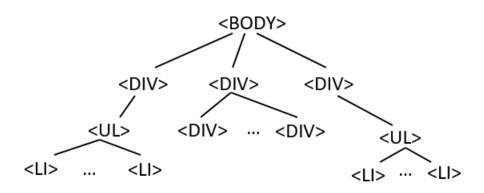
\includegraphics[width=2.5in]{imgs/chap_3/html}} 

\caption{}
\label{fig:Amazon2}
\end{figure*}

 
Figure~\ref{fig:Amazon2} shows an example of the structural and visual representations for the Amazon web page in Fig.~\ref{fig:amazon}. Leafs of the structural tree and the Rendered Block Tree represent the minimum semantic units that cannot be segmented further (e.g., images, plain texts, links).
Actually, the Rendered Block Tree is more complicated than what Figure~\ref{fig:Amazon2}(b) shows (there are often hundreds or even thousands of blocks in a Rendered Block Tree). 


Both Definition \ref{def_chap2:structuralRepresentation} and Definition \ref{def_chap2:visualRepresentation}, which are used to exploit the web page stucture, are used in the definition of web lists, which is crucial for the task of logical list extraction:

\begin{definition}
\label{def_chap2:list}
A \textbf{Web List} is a collection of two or more web elements (called data records) codified as rendered boxes having a similar HTML structure, and visually adjacent and aligned. This alignment can occur via the x-axis (i.e. a vertical list), the y-axis (i.e. horizontal list), or in a tiled manner (i.e. aligned vertically and horizontally)~\cite{Lanotte:2014}. 
\end{definition}

This definition requires an algorithm which is charge of checking whether two rendered boxes ``have a similar HTML structure''. Moreover, it also requires a formal definition of alignment and adjacency. These aspects are discussed in Section \ref{SecChap2:Methodology}.

From the Amazon web page, showed in Fig.~\ref{fig:amazon} it is possible to extract one tiled list (i.e., box A), one horizontal list (i.e., box F) and four vertical lists (i.e., boxed B, C, D, E). 

\begin{definition}
A \textbf{Data Record} identifies an element of a web list. Similar to the concept of data records into database, data records into a web page are a set of similar and structured objects containing information related to a real-world entity. 
\end{definition}

\begin{definition}
\label{def:logicalList}\textbf{Logical List}:
It is a list whose Data Records are distributed on more then one web pages. 
\end{definition}
An example is shown in Fig.~\ref{fig:amazonDiscovery}, where the boxes A1 and A2 represent a part of a \emph{logical list}.
\begin{definition}
\label{def:viewList}\textbf{View List}:
It is a view of a logical list, whose Data Records are all contained in same web page.
\end{definition}
List F in Fig.~\ref{fig:amazon} is an example of a view list. In fact, it contains only some of data records belonging to its logical list (that is the \textit{pagination list}).
\begin{definition}
\label{def:domList}\textbf{Dominant List:} It is the view list of interest, containing data records from the logical list that we want to extract.
%\textbf{Dominant List:} It is the view list of interest, containing the logical list's data records that we want to extract.
\end{definition}
%The list F in Fig.~\ref{fig:amazon} is an example of a view list. In fact it contains only some of data records belonging to its logical list (that is the \textit{pagination list}).
The choose of the dominant list strictly depends on the application goals. For example, if we want extract the whole product listing in an e-commerce website returned by a query, the dominant list is the web list containing products self (i.e. box A in Fig.~\ref{fig:amazon}). However, we could be interested to the navigation systems of a web page. In that case our dominant list could be for example its pagination list (i.e., box F in Fig.~\ref{fig:amazon}).  

%For example the list A in Fig.~\ref{fig:amazon} is the Dominant List for the given Web page.
%Finally in Figure~\ref{fig:amazonDiscovery}, where the boxes A1 and A2 represent a part of a \emph{logical list}.

\section{Methodology}
\label{SecChap2:Methodology}
In this section, I describe the methodology used for \emph{logical list} extraction process. The algorithm employs a three-step strategy.
Let $P$ a web page, it first extracts the set $L^P$ of the lists contained in $P$; in the second step, it identifies the \textit{dominant list} $l_{dom}^P \in L$; finally, it uses $l_{dom}^P$ to discover the \emph{logical list} $LL$ which includes $l_{dom}^P$ as sub-list. 
These steps are detailed in the following sub-sections.

\begin{figure}
\centering
	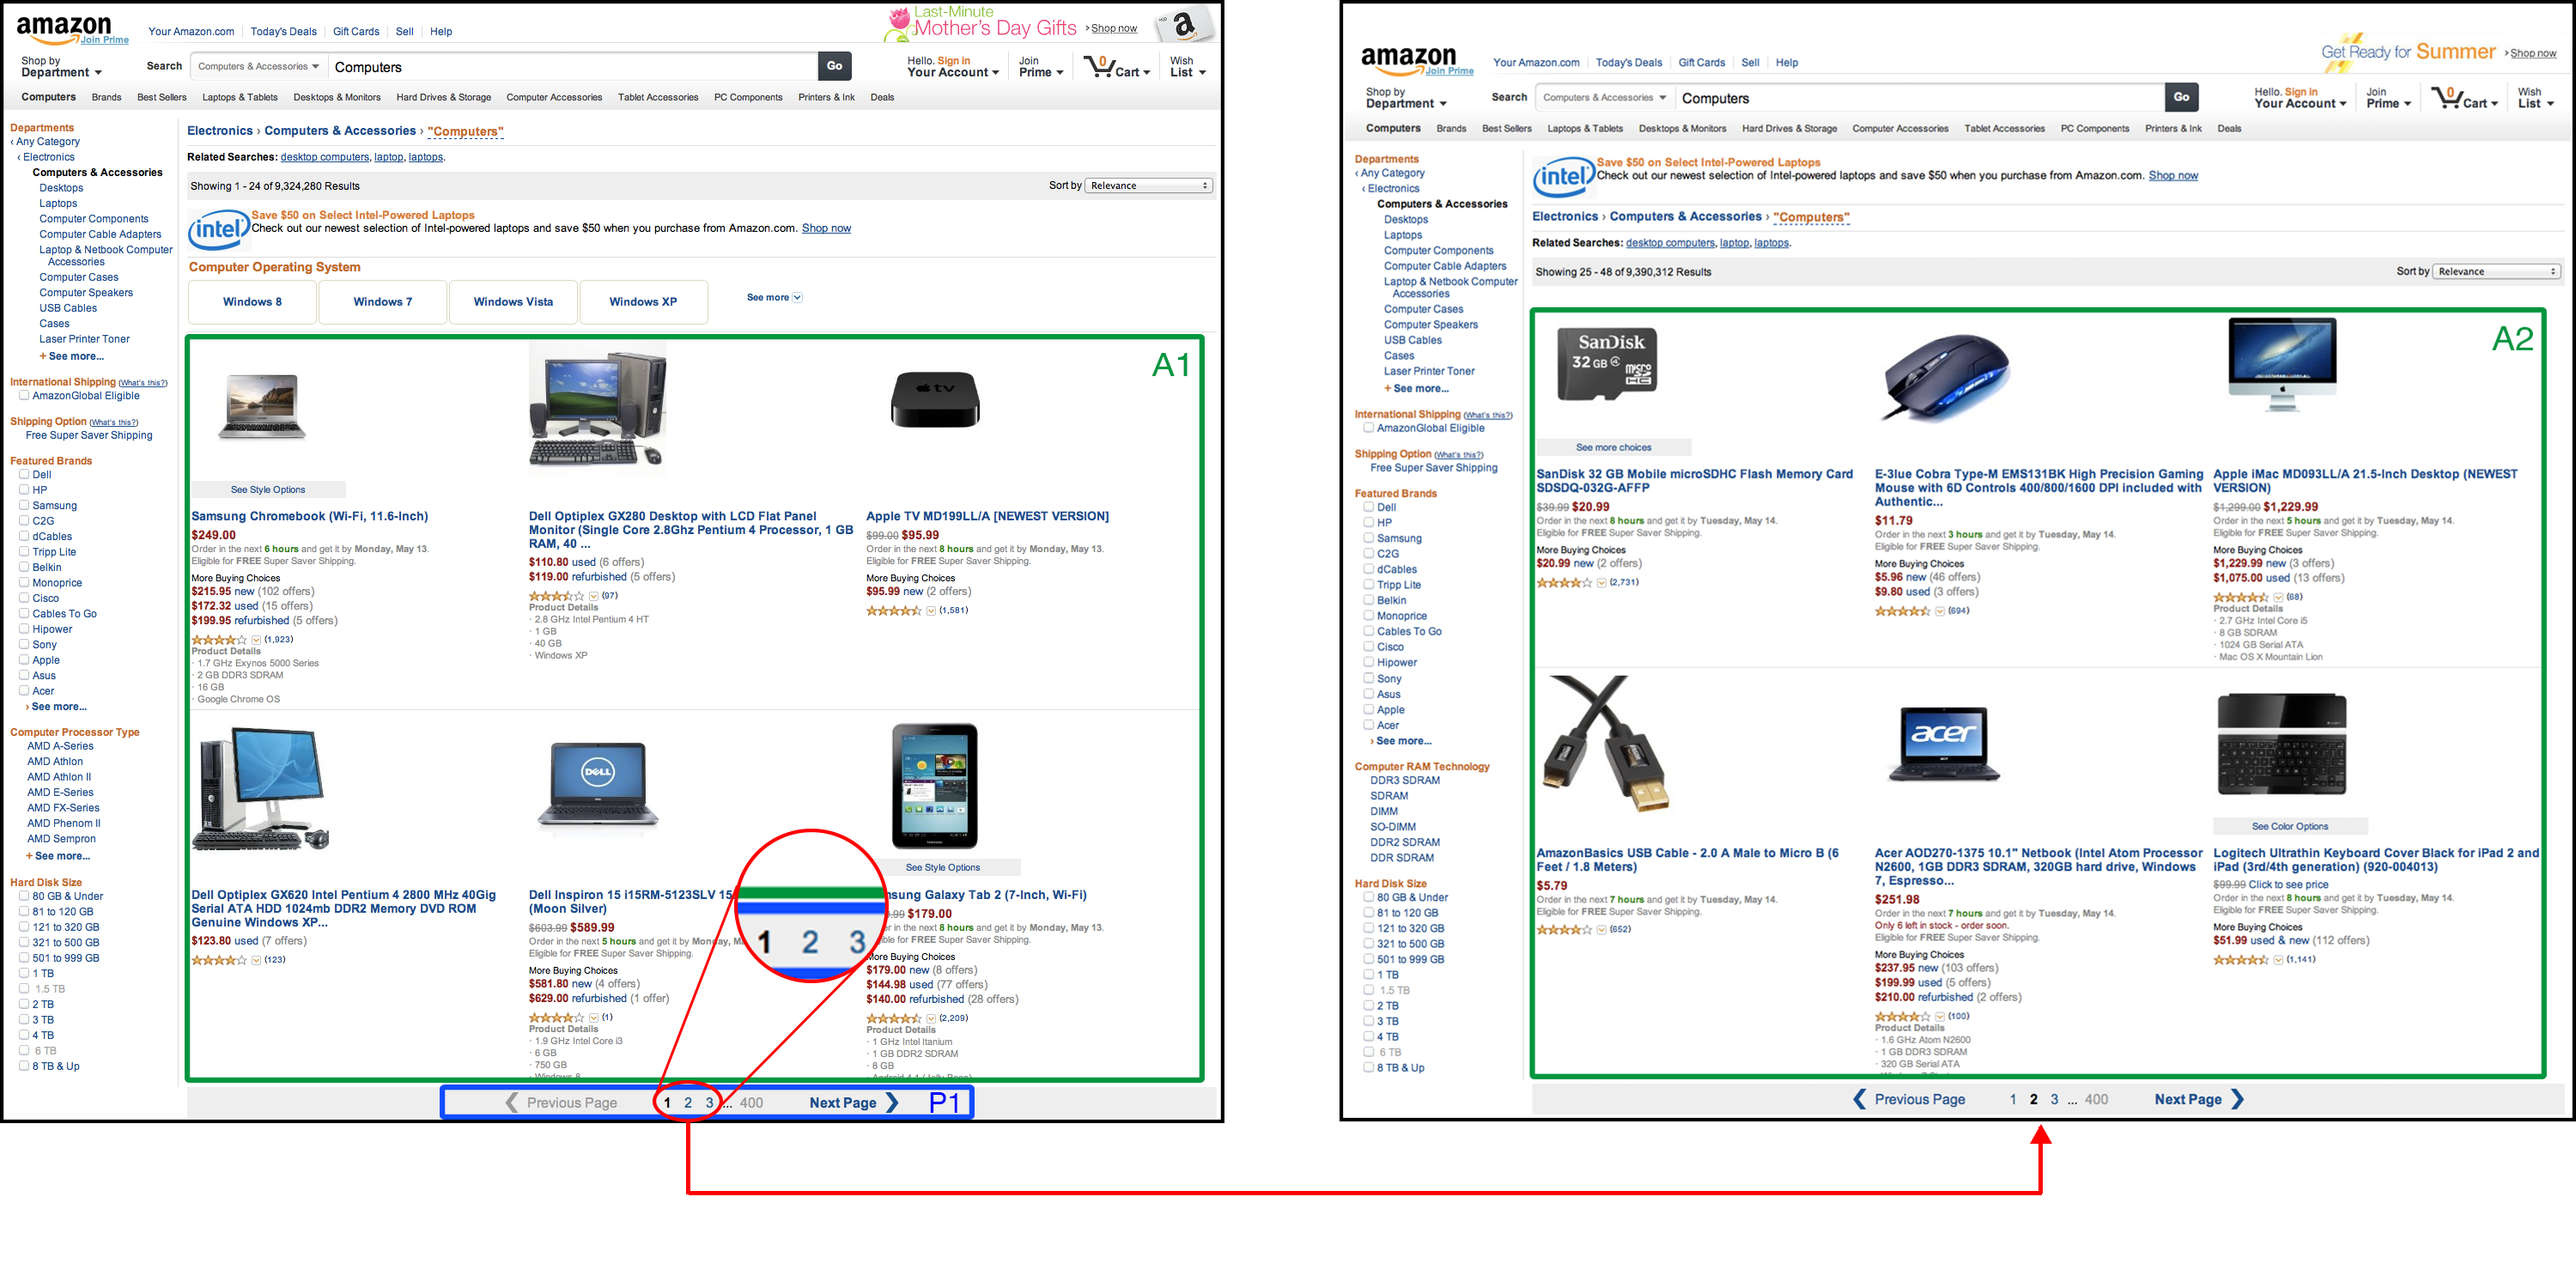
\includegraphics[scale=0.2]{imgs/chap_2/Amazon-discovery.png}
\caption{An example of \emph{logical list} for Amazon's products.}
\label{fig:amazonDiscovery}
\end{figure}

\subsection{List Extraction}
\label{2ListExtraction}
Given a web page $P$ as input, its web lists $L=\{l_1,l_2,\ldots,l_n\}$ are extracted. 
According to Definition \ref{def_chap2:list}, Algorithm \ref{chap2alg:extractWebLists} describes in detail the process of web list extraction. Before to analyze the implementative aspects of this algorithm we need to explore the concepts of \emph{structural similarity}, \emph{adjacency} and \emph{alignment}, between web elements, mentioned in Def.~\ref{def_chap2:list}. 

To check whether two web elements $e_i, e_j$ have similar HTML structure several distance measures can be applied. In the following we describe the measures used, throw this thesis, for computing the structural similarity among web elements:
\begin{itemize}
\item \textit{Normalized Edit Distance}. 
It measures the difference between two strings (or sequences) in terms of the minimum cost needed to transform a string $A$ into the string $B$ (through inserting, deleting or updating operations). This measure is then normalized for the maximum strings' length.
\begin{equation}
NormalizedEditDistance(A,B) = \frac{EditDistance(A,B)}{max(|A|,|B|)}
\end{equation}
For a survey on the Normalized Edit Distance and its variances see~\cite{Yujian:2007}.
For applying the normalized edit distance to two HTML tag trees (web elements) $e_i, e_j$, a conversion step to translate each HTML tag tree into a string format is required. For this scope, each HTML tag in the tree rooted at $e_i$($e_j$) is first codified into a unique character. Then, a string is extracted from the converted tree by applying a breadth search on its nodes. Figure~\ref{fig:NormalizedEditDistance} shows an example of an HTML tag tree rooted at tag $<body>$ and its converted tree. Applying a breadth search to the converted tree, we obtain the string $abbbcbbcdddd$.
Normalized edit distance is suitable to extract web lists whose data records have a simple and a very similar HTML structure (such as most web lists describing websites' navigation systems). To discover more complex web lists, in terms of structural representation, the normalized edit distance can be replaced by the \emph{Normalized Tree Edit Distance}
\item \textit{Normalized Tree Edit Distance.} Similar to the edit distance between strings, the tree edit distance between two trees $A$ and $B$ is the cost associated with the minimum set of operations needed to transform $A$ into $B$. 
Although tree edit distance algorithms are in general computationally more expensive than string edit distance algorithms, they are more accurate to extract web lists whose data records have deep and complex structural representations. %Therefore, if we want extract the product web list of a web page (e.g. box A in Fig.~\ref{fig:amazon}) the Normalized Tree Edit Distance should returns more accurate results than normalized edit distance.
For a survey on the Normalized Tree Edit Distance and its variances see~\cite{Demaine:2009}. For the scope of this thesis I have implemented the Tree Edit Distance proposed in \cite{Zhai:2005} and I have normalized it with the maximum number of nodes contained in $A$ or $B$.
\begin{equation}
NormalizedTreeEditDistance(A,B) = \frac{TreeEditDistance(A,B)}{max(|A|,|B|)}
\end{equation}
\end{itemize}

\begin{figure*}
 \center
\subfloat[Example of an HTML tag tree]{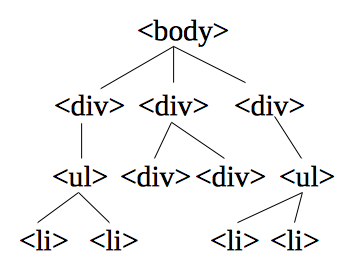
\includegraphics[scale=0.50]{imgs/chap_2/htmlTree.png}} 
\subfloat[Example of a converted HTML tag tree]{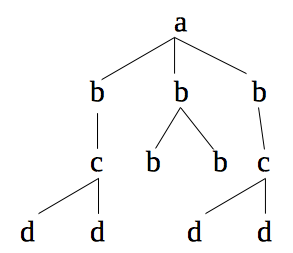
\includegraphics[scale=0.50]{imgs/chap_2/convertedTree.png}}
\caption{}
\label{fig:NormalizedEditDistance}
\end{figure*}
In addition to the structural similarity, other concepts required for the task of web list extraction are those of adjacency and alignment. 
In particular, two web elements $e_i, e_j$ are adjacent if they are siblings in the Rendered Box Tree and there is no  web element $e_w$, with $e_w \neq e_i \neq e_j$, which is rendered between them. Finally, two web elements $e_i, e_j$ are aligned on: \emph{i)} the x-axis if the have same $x$ coordinate, that is $e_i.x = e_j.x$; \emph{ii)} the y-axis if they share the same $y$ value, that is $e_i.y = e_j.y$; \emph{iii)}  both axes, that is $e_i.x = e_j.x$ and $e_i.y = e_j.y$.

After having defined the concepts of structural similarity, adjacency and alignment,  we can describe the method \emph{extractWebLists()} (Algorithm~\ref{alg:extractWebLists}). In particular, the algorithm starts analyzing all the nodes which, in the rendered box tree, are children of the rectangular box representing the \emph{body tag} element (line 2). For each node to analyze (line 4), only if the number of nodes in the subtree rooted in that node is relatively small, the algorithm tries to align its children (lines 9-30). Otherwise, it only enqueues the children for further processing. The rationale is that only small subtrees of the rendered box tree can represent weblists, whereas  subtrees rooted at the higher levels of the rendered box tree typically do not represent any structured data. For the experiments, the threshold value we use for the size of the tree (\emph{maxSize}) is 60. 
Only the nodes which are included neither in \emph{verticalLists} (which contains vertically aligned web elements) nor in \emph{horizontalLists} (which contains horizontally aligned web elements) are further explored by the algorithm (lines 27-28). 
The method \textit{getStructurallySimilar()} is the method that checks whether the elements in a list have similar HTML structure. In this chapter the normalized tree edit distance is applied.

\begin{algorithm}[H]
\caption{extractWebLists(P)}
\label{chap2alg:extractWebLists}
\begin{algorithmic}[1]
\renewcommand{\algorithmicrequire}{\textbf{Input:}}
\renewcommand{\algorithmicensure}{\textbf{Output:}}
\newcommand{\RETURN}[1]{\textbf{return} #1}
\renewcommand{\algorithmiccomment}[1]{$//$ \textit{#1}}
\renewcommand{\algorithmicforall}{\textbf{for each}}
\newcommand{\extractWebLists}[1]{ \textit{extractWebLists}(#1); }
\newcommand{\getChildren}[1]{ \textit{getChildren}(#1);}
\newcommand{\findElementByTagName}[1]{ \textit{findElementByTagName}(#1);}
\newcommand{\dequeue}[1]{ \textit{dequeue}(#1); }
\newcommand{\getVerticallyAligned}[1]{ \textit{getVerticallyAligned}(#1);}
\newcommand{\getHorizontallyAligned}[1]{ \textit{getHorizontallyAligned}(#1);}
\newcommand{\getStructurallySimilar}[1]{ \textit{getStructurallySimilar}(#1)}
\newcommand{\getNotAligned}[1]{ \textit{getNotAligned}(#1);}
\newcommand{\add}[1]{ \textit{add}(#1); }
\newcommand{\enqueue}[1]{ \textit{enqueue}(#1); }
\newcommand{\getUrls}[1]{ \textit{getUrls}(#1) }
%\SetKwFunction{FMain}{Main}
\REQUIRE web page P;
\ENSURE List$<$List$<$Web elements$>>$ L; //list of weblists.
\STATE body = webpage.\findElementByTagName{''body''}
\STATE notAligned = body.\getChildren{}
\REPEAT 
	
	\STATE node = notAligned.\dequeue{}
	\STATE children = node.\getChildren{}
	
	\IF{ node.getSize() $>=$ maxSize}
	\STATE notAligned.\enqueue{children}
	\ELSE 
	%\STATE verticalLists = children.groupBy(c $\rightarrow$ c.x)
	%\\.map(list $\rightarrow$ \getStructurallySimilar{list}) 
	%\\.filter(list $\rightarrow$ list.size $\geq$ 2)
    \STATE verticalAligned= children.groupByX();
    \STATE horizontalAligned = children.groupByY();
    
    \FORALL{list $\in$ verticalAligned}
    \STATE structurallySimilar = getStructurallySimilar(list);
    \IF{ structurallySimilar.getSize() $\geq$ 2}
    \STATE L.add(structurallySimilar);
    \ENDIF
	\ENDFOR 
	
	\FORALL{list $\in$ horizontalAligned}
    \STATE structurallySimilar = getStructurallySimilar(list);
    \IF{ structurallySimilar.getSize() $\geq$ 2}
    \STATE L.add(structurallySimilar);
    \ENDIF
	\ENDFOR 
	
	\STATE notIncluded = children - lists.getWebElements();
	\STATE notAligned.\enqueue{notIncluded}
	\ENDIF


\UNTIL{!notAligned.empty()}
\RETURN{L}


\end{algorithmic}
\end{algorithm}

\subsection{Dominant List Identification}

Given a web page $P$ and the set of list $L=\{l_1,l_2,\ldots,l_n\}$ extracted in the first step, three measures are used to identify the \textit{dominant list} of P: 
\begin{itemize}
\item \textbf{Centrality.} Given a list $l_i \in L$, the \emph{centrality} of $l_i$ w.r.t P is obtained by computing the Euclidean distance between the center of the parent-box of $l_i$ and the center of root-box of $P$.
\item \textbf{Area Ratio.} Given a list $l_i \in L$, the \emph{area ratio} of $l_i$ w.r.t P is the size of the box containing $l_i$ divided the size of root-box of $P$.
\item \textbf{Text-Tag Ratio.}  Given a list $l_i \in L$, and let $m$ the length of $l_i$, the \emph{text-tag ratio} of $l_i$ is computed as:
\begin{equation}
 \frac{1}{m}\sum_{j=0}^m \frac{chars(l_i[j])}{tag(l_i[j])}
\end{equation}
where $tag(l_i[j])$ is the number of HTML tags contained in the j-th data record of $l_i$ and $chars(l_i[j])$ is the total number of characters contained in $l_i[j]$. 
Before that the text-tag ratio is computed, \textit{script} and \textit{remark} tags
are removed because this information should be not considered in the count of non-tag text. 
\end{itemize}
In particular the \textit{Dominant list} of P is the list with  the highest sum of contributions:
\begin{equation}
\argmax_{{l_i \in L}} \frac{\alpha_1}{centrality(l_i)} + \alpha_2areaRatio(l_i)+ \alpha_3textTagRatio(l_i)
\end{equation}
where $centrality(l_i), areaRatio(l_i)$ and $textTagRatio(l_i)$ are respectively the centrality measure, area ratio and text-tag ratio of a list $l_i$ contained in L. $\alpha_1=\alpha_2=\alpha_3$ are set to $0.3$ to give the same weight to each measure.

%\begin{algorithm}
%\caption{\texttt{LogicalListDiscovery}}\label{alg:lld}
%
%\begin{algorithmic}[1]
%%\SetKwInOut{Input}{input}
%%\SetKwInOut{Output}{output}
%\renewcommand{\algorithmicrequire}{\textbf{Input:}}
%\renewcommand{\algorithmicensure}{\textbf{Output:}}
%\REQUIRE{ dominant list $l_{dom}^P$, set $L_{-}=\{L \setminus l_{dom}^P\}$}
%\ENSURE{ logical list $LL$}
%%\Input{ dominant list $l_{dom}^P$, set $L_{-}=\{L \setminus l_{dom}^P\}$}
%%\Output{ logical list $LL$}
%%\BlankLine
%		\STATE $LL = \{l_{dom}^P\}$%\;
%		\FORALL{$l \in L_{-}$}
%			\FORALL{$u \in l$}
%				$L_u \gets$ HyLiEn$(u)$%\;
%				$L_u$.filterSimilarity($l_{dom}^P,\alpha$)%\;
%				$LL$.add($L_u$)%\;
%	  \STATE $LL \gets LL$.flatMap()%\;
%	  \STATE $LL \gets LL$.removeDuplicates()\;
%	  \RETURN {$LL$}%\;
%\end{algorithmic}
%\end{algorithm}

\begin{algorithm}
\caption{\texttt{LogicalListDiscovery}}\label{alg:lld}

\begin{algorithmic}[1]
%\SetKwInOut{Input}{input}
%\SetKwInOut{Output}{output}
\renewcommand{\algorithmicrequire}{\textbf{Input:}}
\renewcommand{\algorithmicensure}{\textbf{Output:}}

\REQUIRE dominant list $l_{dom}^P$, set $L_{-}=\{L \setminus l_{dom}^P\}$
\ENSURE logical list $LL$
\STATE $LL = \{l_{dom}^P\}$
\FORALL{$l \in L_{-}$}
	\FORALL{$u \in l$}
		\STATE $L_u \gets$ HyLiEn$(u)$
		\STATE $L_u$.filterSimilarity($l_{dom}^P,\alpha$)%\;
		\STATE $LL$.add($L_u$)%\;
		\ENDFOR
		\ENDFOR

\STATE $LL \gets LL.$flatMap()%\;
\STATE $LL \gets LL$.removeDuplicates()%\;
\STATE \textbf{return} $LL$%\;
		
\end{algorithmic}
\end{algorithm}

\subsection{Logical List Discovery}
Identified the dominant list $l_{dom}^P$ of the web page P, the last step of the algorithm is to discover the logical list $LL$ containing $l_{dom}^P$. This is done by taking advantage of the regularities of wesites. As described by Crescenzi et al.~\cite{Crescenzi:2005}, web page links reflect the regularity of the web page structure. In other words, links that are grouped in collections with a uniform layout and presentation usually lead to similar pages. Link-based approaches are used in the literature for tasks strictly related to the one solved by our method. For instance, Lin et al.~\cite{Lin:2010} used web links to discover new attributes for web tables by exploring hyperlinks inside web tables. Lerman et al.~\cite{Lerman2004} uses out-links to ``detail web pages'' in order to segment web tables. In this champter, I successfully use links grouped as lists to navigate web pages and to discover \textit{logical lists}.
\color{black}

Algorithm~\ref{alg:lld} describes the approach used. It takes as input the dominant list $l_{dom}^P$, the minimum similarity threshold $\alpha$, and the set of the lists $L$ extracted from $P$. It iterates over all the lists in the set $L_{-}=\{L \setminus l_{dom}^P\}$ (line 1), and, for each url $u$ in $l_i$ it alternates, (i) the extraction of the set list $L_u$ contained in the web page $U$ having $u$ as url (line 4) to, (ii) the filtering of all the lists in $L_u$ which have a similarity with $l_{dom}^P$ lower than $\alpha$ (line 6). At each iteration, all the lists resulting from step (ii) are added to LL (line 7). Finally, LL is flattened and all the duplicate elements are merged (lines 8-9). 
Moreover, during the process all the anchor text of url $u$ are used as attributes to annotate the discovered \emph{view} lists and are reported in the final \emph{logical list} $LL$.
\section{Experiments}
In this section I present the empirical evaluation of the proposed algorithm. For this scope, a test dataset is manually generated and verified. In particular, for the experiment, I select 40 websites in different application domains (music shops, web journals, movies information, home listings, computer accessories, etc.) with list elements presented in different ways. For the deep-web databases, I performed a query for each of them and collected the first page of the results list;  for others website I manually selected a random web page. Table 1 shows in the first column the ground truth, that is, the number of data records which belong to the \textit{logical list} to be extracted.
The dataset is composed of 66.061 list elements extracted from 4405 web pages. In particular, the following steps are carried out to extract from an input page its logical list: (i)  the web page is rendered in a web browser, (i) the \emph{dominant list} is manually identified and its data records are included in the logical list, and (ii) the \emph{logical list} is enriched following the out-links of the other lists in the page. This task required around 7 days of 4 people.


%We rendered each Web page and we manually identified (i) \emph{dominant list} and, (ii) following the out-links of the other lists in the pages we annotated \emph{logical lists}. This task required around 7 days of 4 people.

To the best of my knowledge the task of \emph{Logical List Discovery} is novel, and there are not any other methods to compare with. So, I evaluated the effectiveness of our algorithm by using \emph{precision}, \emph{recall} and \emph{f-measure} metrics, computed over the number of \emph{logical list} elements to be extracted (manually verified) w.r.t to the algorithm results. In particular, the precision is the measure of, how many of the extracted \emph{view} lists belong to a \emph{logical list}. The recall allows us to measure how many of the discovered \emph{view} lists are true positive element of a \emph{logical list}. i also included the \emph{F-Measure} which is the weighted harmonic means of \emph{precision} and \emph{recall}. 
These metrics are evaluated counting how many data records of the \emph{logical list} are found in the \emph{view} lists.
\begin{equation}
precision= \frac{TP}{TP + FP},~
recall= \frac{TP}{TP + FN},\\
F-measure= \frac{2(precision \times recall)}{precision + recall}
\end{equation} 

\subsection{Results}
The execution of the algorithm requires two parameters which are empirically set to $\alpha=0.6$ and $\beta=50$. These parameters are need by the HyLiEn Algorithm. Our methods uses $\alpha$ during the \emph{Logical List Discovery} step.

Table 1 presents the main results. The first column holds for each logical list the number of data records to extract. The second and the third columns contain the number of true positive and the number of false negatives data records. I do not plot the number of false positives, because our algorithm outputted always 0 false positives during the experiment evaluation. Finally, the fourth, fifth and sixth columns show the values for precision, recall and f-measure.

In general, the experimental results show that our algorithm is able to discover \textit{logical lists} in a varying set of websites (that is, it is not domain dependent). Moreover, the quality of the results are not correlated to how the lists are rendered in web pages (i.e. horizontal, vertical and tiled). In average, it achieves $100\%$ for Precision, $95\%$ for Recall and a F-Measure $97\%$. With respect to the ground truth, the algorithm does not extract any False Positive, and it outputs only 466 False Negatives. 
In general, it returns perfect results ($100\%$ precision and recall) for several kind of websites spanning different applications domain, but there are some of them which presents values for recall ranging from $81\%$ and $91\%$. Considering ``last.fm'', which gave a recall equal to $81\%$, I found that the presentation of the data records is sometime quite different, because of the high variance in the number of the ``similar to'' tags (which are presented as HTML $<$a$>$ ) assigned to each listing. Analyzing other examples such as ``IlSole24Ore.it'' and ``RealEstateSource.au'' we found the same problem, that is, the presentation of the data records is quite variable across the web pages, and so the HyLiEn algorithm sometimes misses some of the data records. Anyway we see that the proposed algorithms is effective is able to discover \emph{logical lists} on different type of websites.

\begin{table}%[!htb]
 \centering
 \begin{tabular}{|l|c|c|c|c|c|c|}
  \hline
  \hline
  \textbf{Website} & $Ground$ & $TP$ & $FN$ & $Precision$ & $Recall$ & $F\text{-}measure$ \\
  \hline
  BariToday.it & 904 & 904 & 0 &100\% & 100\% & 100\% \\
  \hline
  Subito.it & 1000 & 1000 & 0 & 100\% & 100\% & 100\% \\
  \hline
  GitHub.com & 100 & 100 & 0 & 100\% & 100\% & 100\% \\
  \hline
  TestoLegge.it & 360 & 360 & 0 & 100\% & 100\% & 100\% \\
  \hline
  Zoopla.co.uk & 597 & 597 & 0 & 100\% & 100\% & 100\% \\
  \hline
  FindAProperty.co.uk & 60 & 60 & 0 & 100\% & 100\% & 100\% \\
  \hline
  Savills.co.uk & 232 & 232 & 0 & 100\% & 100\% & 100\% \\
  \hline
  AutoTrader.co.uk & 60 & 60 & 0 & 100\% & 100\% & 100\% \\
  \hline
  EbayMotors.com & 3925 & 3925 & 0 & 100\% & 100\% & 100\% \\
  \hline
  Doogal.co.uk & 38240 & 38240 & 0 & 100\% & 100\% & 100\% \\
  \hline
  RealEstateSource.com & 368 & 316 & 62 & 100\% & 85\% & 91\% \\
  \hline
  AutoWeb.co.uk & 180 & 180 & 0 & 100\% & 100\% & 100\% \\
  \hline
  TechCrunch.com & 434 & 422 & 12 & 100\% & 95\% & 98\% \\
  \hline
  Landsend.com & 1243 & 1243 & 0 & 100\% & 100\% & 100\% \\
  \hline
  TMZ.com & 300 & 300 & 0 & 100\% & 100\% & 100\% \\
  \hline
  IlSole24Ore.it & 510 & 445 & 65 & 100\% & 81\% & 86\% \\
  \hline
  GoBari.it & 350 & 340 & 10 & 100\% & 97\% & 98\% \\
  \hline
  AGI.it & 60 & 60 & 0 & 100\% & 100\% & 100\% \\
  \hline
  BBCNews.co.uk & 347 & 310 & 37 & 100\% & 89\% & 94\% \\
  \hline
  milano.corriere.it & 30 & 30 & 0 & 100\% & 100\% & 100\% \\
  \hline
  torino.repubblica.it & 70 & 68 & 2 & 100\% & 98\% & 99\% \\
  \hline
  Ansa.it & 1506 & 1479 & 27 & 100\% & 98\% & 99\% \\
  \hline
  LeMonde.fr & 445 & 418 & 27 & 100\% & 94\% & 97\% \\
  \hline
  Time.com & 377 & 377 & 0 & 100\% & 100\% & 100\% \\
  \hline
  aur.ArchLinux.org & 575 & 575 & 0 & 100\% & 100\% & 100\% \\
  \hline
  Immobiliare.it & 609 & 536 & 73 & 100\% & 86\% & 93\% \\
  \hline
  bitbucket.org & 130 & 130 & 0 & 100\% & 100\% & 100\% \\
  \hline
  MyMovies.com & 563 & 515 & 48 & 100\% & 92\% & 96\% \\
  \hline
  Trulia.com & 3300 & 3300 & 0 & 100\% & 100\% & 100\% \\
  \hline
  YouTube.com & 580 & 567 & 13 & 100\% & 98\% & 99\% \\
  \hline
  FileStube.com & 332 & 304 & 28 & 100\% & 91\% & 95\% \\
  \hline
  Last.fm & 60 & 41 & 19 & 100\% & 68\% & 81\% \\
  \hline
  Bing.com & 130 & 130 & 0 & 100\% & 100\% & 100\% \\
  \hline
  addons.mozilla.org & 984 & 939 & 45 & 100\% & 95\% & 97\% \\
  \hline
  AutoScout24.com & 840 & 840 & 0 & 100\% & 100\% & 100\% \\
  \hline
  Facebook.com & 2820 & 2820 & 0 & 100\% & 100\% & 100\% \\
  \hline
  SlideShare.net & 2037 & 2037 & 0 & 100\% & 100\% & 100\% \\
  \hline
  Gazzetta.it & 970 & 970 & 0 & 100\% & 100\% & 100\% \\
  \hline
  ElPais.es & 294 & 285 & 9 & 100\% & 98\% & 99\% \\
  \hline
  StackOverflow & 585 & 585 & 0 & 100\% & 100\% & 100\% \\
  \hline
  \hline
  Sums and  Averages & 66.527 & 66.061 & 466 & 100\% & 95\% & 97\% \\
  \hline
  \end{tabular}
 \label{table:results}
 \caption{Discovered \emph{logical list} elements for websites dataset.}
\end{table}
